\section{Performance Evaluation}
The extension's performance goals are to provide our security guarantees without being a detriment to the end user's browsing experience. All of our timestamps were recorded using the Performance Web API. While our extension's functionality only applies at the network level, there is potential slowdown at the DOM processing level. Figure ~\ref{fig:navigationtiming} presents shows the different timestamps provided by the Navigation Timing API, as well as a high-level description of the browser processing model. Since our filter listens on the onBeforeRequest event, none of the previous steps before Request are affected. In this section, we refer to the difference in time between responseEnd and requestStart as the "network filter time".

\begin{figure}[h]
 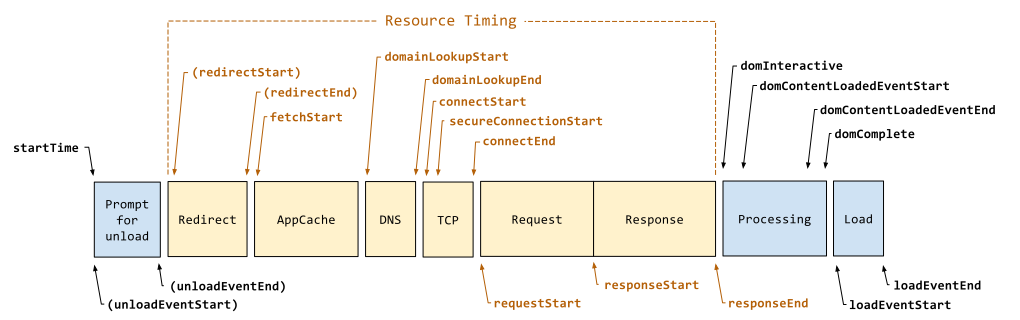
\includegraphics[scale=0.32]{img/timestamp-diagram}
 \caption{The Navigation Timing API's timestamps}
 \label{fig:navigationtiming}
 \end{figure}

\subsection{Top websites load times}
We first report our extension's impact on top website load times, representing the expected behaviour of an user's average web browsing experience. For these tests, we first took the top 500 websites as reported by Moz.com \cite{top500}. For each website, we loaded it 20 times (with a 25 second timeout) and recorded the following values: requestStart, responseStart, responseEnd, domContentLoadedEventEnd, domComplete, duration, and decodedBodySize. From the initial 500, we only report values for 441 of them. The other 59 had consistent issues with timeouts, insecure certificates, and network errors. For our setup, we used a headless version of Firefox, and Selenium WebDriver for NodeJS, with GeckoDriver. We ran four test suites:
\begin{itemize}
	\item No extension cold cache: Firefox is loaded without the extension installed and the web driver is re-instantiated for every page load.
	\item Extension cold cache: Firefox is loaded with the extension installed and the web driver is re-instantiated for every page load.
	\item No extension warm cache: Firefox is loaded without the extension installed and the same web driver is used for the page's 20 loads.
	\item Extension warm cache: Firefox is loaded with the extension installed and the same web driver is used for the page's 20 loads.
\end{itemize}

The recorded timestamps do not hold much value by themselves, only when analysed with regards to each other. Thus, for each set of tests, we reduced the recorded values to three comparisons: responseStart (responseStart-requestStart), responseEnd (responseEnd-requestStart), and domResponse(domComplete-responseStart). The first two analyze the time spent by the network filter, while the third determines the time spent until the whole document has loaded. We calculate the medians of each website for each of the previous three values and the decodedByteSize.

Finally, we compare the load times with and without the extension running by calculating the relative slowdown with the extension installed. Figure ~\ref{fig:overall_slowdown} shows the computed results. The graph shows that the slowdown is not too great when the extension is running. Note that these values are recorded as percentages, and while some are as high as 200\%, the absolute values are in the order of seconds, and in many cases tens or hundreds of milliseconds, especially for the network component. The slowdown increases when we take caching into account. We expect this to be the case because the network filter probably causes the browser to use less caching, especially for the DOM component, as it might have to process it from scratch every time.

Figure ~\ref{fig:histogram_slowdown} shows a closer look at the distribution for the network filter slowdown on the top sites. We see that for this component, most of the slowdown is centred around [-10\%,10\%].

Figure ~\ref{fig:network_filter_decoded_size} shows the network filter time as a function of the page's decoded byte size. Since the probes perform regex matching, the upwards trend line is expected. However, we see that almost all the sites up to 1.2 MB take under 500 ms.


\begin{figure}[h]
	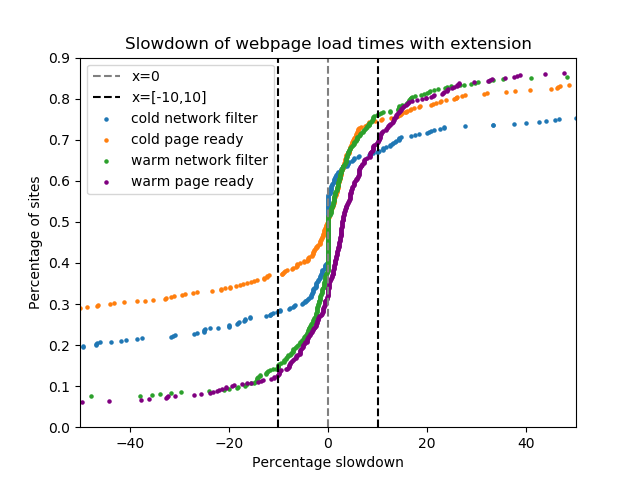
\includegraphics[scale=0.5]{results/extension_slowdown_overall}
	\caption{Cumulative distribution of relative percentage slowdown with extension installed for top sites}
	\label{fig:overall_slowdown}
\end{figure}

\begin{figure}[h]
	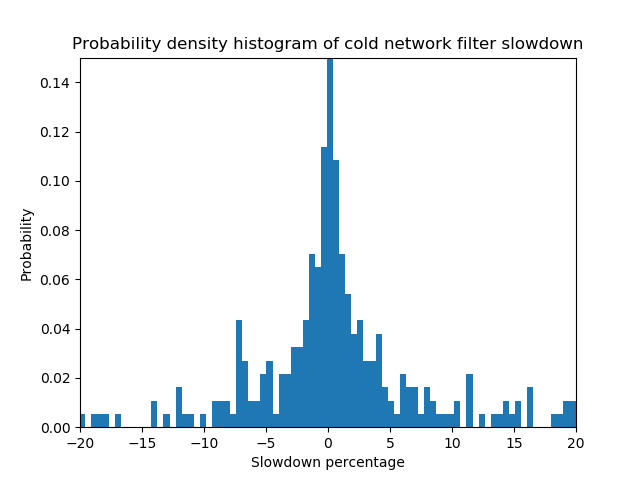
\includegraphics[scale=0.5]{results/density_histogram_filter_slowdown}
	\caption{Density histogram of network filter slowdown for top sites}
	\label{fig:histogram_slowdown}
\end{figure}

\begin{figure}[h]
	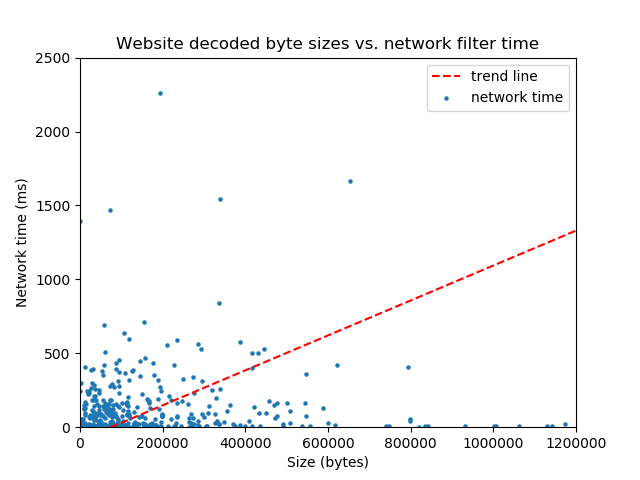
\includegraphics[scale=0.5]{results/byte_size_vs_filter_time}
	\caption{Scatter plot of network filter time as a function of decoded byte size for top sites}
	\label{fig:network_filter_decoded_size}
\end{figure}

